\chapter{Implementation}
% (more or less telling whats in my code; implementation details; describing dataset; which network and which hyper parameters do I use; how does the application look like)
\section{Setup}

Remote PC for Learning

Major frameworks and their respective versions:
Tensorflow:    tensorflow-gpu==1.14.0
               tensorboard==1.14.0
Keras: 2.3.1
Python: 3.6
MTCNN: 0.1.0
keras-vggface: 0.6


Command Line access:

Jupyter Notebook access to remote server:
For remoteuser@remotehost:
\begin{itemize}
    \item remoteuser@remotehost:
    jupyter notebook --no-browser --port=XXXX
    
    \item localuser@localhost:
    ssh -N -f -L localhost:YYYY:localhost:XXXX -L localhost:ZZZZ:localhost:WWWW remoteuser@remotehost
    (ZZZZ is port at local machine for the tensorboard, while WWWW represents the port on the remote machine on which tensorboard is running)
    
    \item localuser@localhost:
    http://localhost:YYYY
\end{itemize}
The jupyter notebook is being started up through running the 'localhost:YYYY' command in the web browser, while the tensorboard is started through the following command inside the jupyter notebook 'tensorboard --logdir <path> --port ZZZZ'

\section{Dataset}
Which dataset did I use for training and testing?
If AFEW-VA , then cite the paper and write sth. about it.
\cite{Kossaifi:2017:AFEW-VADatabase}
\cite{Dhall:2012:AFEWVA}
(two sources from README)

-> Structure of data
each video clips is split into multipe frames. All these frames are kept into one folder.
-> Structure of labels
Each folder with the respective frames for the video clip have a .json file named according the naming schema for the folders, e.g. folder name is '001' then the file for the labels will have the name '001.json'. This file contains for each frame a label/value for the emotional values of valence and arousal. Additionally it also includes the pre-labeled landmarks for face detection purposes. These landmarks are as of now (5th of July 2020) not utilized, as an external module is being used for the face detection task.

\begin{quote}
    To compare the performance of various features, we sampled regularly an equal number of frames from each sequence to obtain a set of frames representative of the whole dataset, which we then divided in 5 disjoint folds in a subject-independent manner (i.e. a subject does not appear in two different folds). We then performed a 5-fold cross-validation (i.e. we iteratively used one of the set for testing and the other 4 for training) to predict the valence and arousal values for each frame\cite{Kossaifi:2017:AFEW-VADatabase}
\end{quote}

\section{Architecture}

\begin{figure}[H]
  \begin{center}
  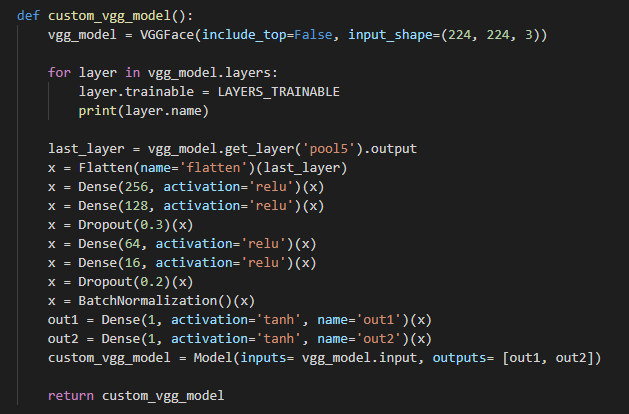
\includegraphics[angle=0, width=0.9\textwidth]{Figures/model_architecture.PNG}
  \caption{Architecture: Custom ML Model}
  \label{fig:ArchitectureCustomMLModel}
  \end{center}
\end{figure}

The model is using the X number of layers from the VGGFace model which layers can be either trained or not, depending on the purpose. The output of the last Pooling layer, after all the Convolutional layers, is being taken and used as an input into the custom built model.

The custom model consists firstly, of a Flatten layer bring the previous output in a fitting shape. Following this, there are 4 Dense layers with different numbers of parameters which decrease, so that information gets more and more crystallized towards the desired output. In between there are two Dropout layers and one BatchNormalization layer which are common techniques to prevent a ML Model from overfitting. Thus, using these techniques, the model can still perform well on a validation dataset.
\newline\newline
The output is split up into two variables which are defined by an Dense layer with activation 'tanh'. This split is necessary, because the metrics can then be applied to each of the outputs separately.
\newline\newline
Architecture strategy:
\begin{quote}
    The experiments in the paper 'Comparison of Fine-Tuning and Extension Strategies for Deep Convolutional Neural Networks' \cite{Pittaras:2017:FineTuningStrategiesComparison} show that the method of increasing the depth of a pre-trained network with one fully-connected layer and fine-tuning the rest of the layers on the target dataset can improve the network’s concept detection accuracy, compared to other fine-tuning approaches
\end{quote}


\section{Metrics}
The accuracy metric is a standard metric in Machine Learning, it tells you about the number of correctly predicted data points out of all data points. In a regression problem, like in this instance, it represents the percentage of how good the predicted values match the actual values.
\newline\newline
RMSE (Root-mean-squared error) and CORR (Pearson product-moment correlation coefficient) are the most commonly found metrics for Emotion Recognition challenges. 

\begin{quote}
    CORR gives information about the magnitude of the association, or correlation, as well as the direction of the relationship. \cite{2020:PearsonCorrelation}
\end{quote}

\begin{quote}
    Root Mean Square Error (RMSE) is the standard deviation of the residuals (prediction errors). Residuals are a measure of how far from the regression line data points are ... In other words, it tells you how concentrated the data is around the line of best fit. \cite{2020:RMSE}
\end{quote}

To sum it up, RMSE lets the observer grasp how exact the predicted value is, while CORR tells you how strong the relationship between prediction and label is.

\begin{figure}[H]
  \begin{center}
  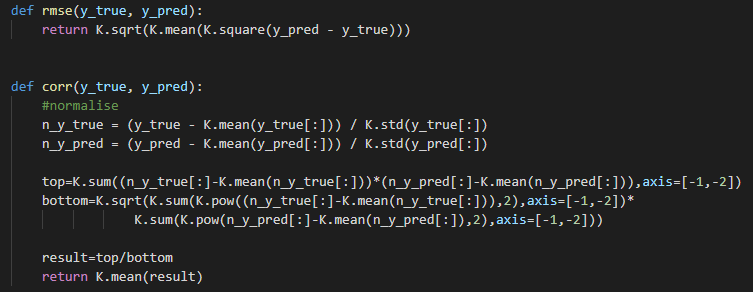
\includegraphics[angle=0, width=0.9\textwidth]{Figures/model_metrics.PNG}
  \caption{Model Custom Metrics}
  \label{fig:ModelCustomMetrics}
  \end{center}
\end{figure}

\section{Regularization}
This post covered a lot of topics, but hopefully you now have an idea of the basics of modeling, overfitting vs underfitting, bias vs variance, and model optimization with (cross-validation). \cite{Koehrsen:2018:OverfittingVSUnderfitting}

Prevention overfitting
https://elitedatascience.com/overfitting-in-machine-learning
\newline\newline
Another source:
Reducing overfitting through applying regularization to pretrained neural networks
https://sthalles.github.io/keras-regularizer/
\newline\newline
Callbacks: 
- Checkpoint for Best Model
- EarlyStopping
- Reduce Learning Rate on Plateau
- Lambda Calback: Setting the layers from the VGGFace model to trainable, for further fine-tuning, after a few epochs of training.

\begin{figure}[H]
  \begin{center}
  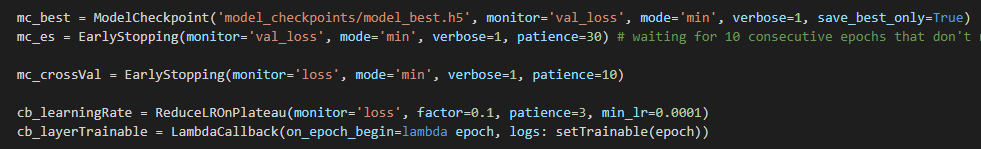
\includegraphics[angle=0, width=0.9\textwidth]{Figures/model_callbacks.PNG}
  \caption{Callbacks for the training process}
  \label{fig:CallbacksTraining}
  \end{center}
\end{figure}

When training I injected callbacks into the training function. These callbacks allow me to keep track of the best model and automatically saves this model according to a specified metric which is in this case the validation loss.\newline
Moreover, a second checkpoint, called 'EarlyStopping', is used to make the model step as soon as it is clear that no improvement is made and saves the last model. The early stopping checkpoint is waiting for 30 consecutive epochs during which a certain specified variable is not improving. In this instance, this checkpoint again is looking at the validation loss as the variable to be observed.

ReduceLearningRateOnPlateau = a checkpoint that automatically reduces the learning rate by a certain factor once it detects that a monitored variable is not improving for a certain period of epochs.

LambdaCallback is a custom callback function used in this case to execute a function on the beginning of each epoch. In this case, 


	